\documentclass{article}
\usepackage{verbatim}
\usepackage{titlesec}

\def\coursename{STAT 447C: Bayesian Statistics}
\def\semester{Fall 2024}

\setlength{\oddsidemargin}{0.0 in}
\setlength{\evensidemargin}{0.0 in} 
\setlength{\topmargin}{-0.6 in} 
\setlength{\textwidth}{6.5 in} 
\setlength{\textheight}{8.5 in}
\setlength{\headsep}{0.75 in} 
\setlength{\parindent}{0 in}
\setlength{\parskip}{0.1 in}

\titleformat*{\section}{\Large\bfseries}


% prints box at top of first page with relevant info
\newcommand{\problemset}[3]{
   \pagestyle{myheadings}
   \thispagestyle{plain}
   \newpage
   \noindent
   \begin{center}
   \framebox{
      \vbox{\vspace{2mm}
    \hbox to 6.28in { {\bf \coursename
                        \hfill \semester} }
       \vspace{4mm}
       \hbox to 6.28in { {\Large \hfill #3  \hfill} }
       \vspace{2mm}
       \hbox to 6.28in { {\it #1 \hfill \texttt{#2}} }
      \vspace{2mm}}
   }
   \end{center}
   \vspace*{4mm}
}

\newcommand{\qsol}[1]{\section{#1}}
  % DO NOT CHANGE
% \usepackage{graphicx,amssymb,amsmath,amsthm,mathrsfs}
% \usepackage{multirow,makeidx,algorithmic,algorithm}
\usepackage{multirow,makeidx,algpseudocode,algorithm}
\usepackage{mathtools}
\usepackage{enumitem}
 
\usepackage{parskip}
\usepackage{setspace}
\usepackage{float, graphicx}
\usepackage{adjustbox}
\usepackage{bbm}
\usepackage{tabularx}
\usepackage{subfigure}
\usepackage{amsmath,amssymb,amsfonts,amsthm,amsbsy,amstext,mathrsfs}
\usepackage{hyperref}
\usepackage{url}
\usepackage{color}
\usepackage{graphicx} % Required for inserting images
\usepackage[utf8]{inputenc}

%% reference
\usepackage[round]{natbib}
\bibliographystyle{abbrvnat}
% \usepackage{cite}
% \bibliographystyle{plainurl}
% \bibliographystyle{abbrv}
% \bibliographystyle{plain}
% \bibliographystyle{unsrt}


%% code in-text
\usepackage{listings}
\usepackage{xcolor}

\definecolor{codegreen}{rgb}{0,0.6,0}
\definecolor{codegray}{rgb}{0.5,0.5,0.5}
\definecolor{codepurple}{rgb}{0.58,0,0.82}
\definecolor{backcolour}{rgb}{0.95,0.95,0.92}

\lstdefinestyle{mystyle}{
    backgroundcolor=\color{backcolour},   
    commentstyle=\color{codegreen},
    keywordstyle=\color{magenta},
    numberstyle=\tiny\color{codegray},
    stringstyle=\color{codepurple},
    basicstyle=\ttfamily\footnotesize,
    breakatwhitespace=false,         
    breaklines=true,                 
    captionpos=b,                    
    keepspaces=true,                 
    numbers=left,                    
    numbersep=5pt,                  
    showspaces=false,                
    showstringspaces=false,
    showtabs=false,                  
    tabsize=2
}

\lstset{style=mystyle}


%% layout
\oddsidemargin 3mm
\evensidemargin 3mm
\topmargin -12mm
\textheight 660pt
\textwidth 450pt  % DO NOT CHANGE
% ADD YOUR CUSTOM NOTATION HERE
\newcommand{\R}{\mathbb R}
\newcommand{\Z}{\mathbb Z}
\newcommand{\Q}{\mathbb Q}
\newcommand{\N}{\mathbb N}
\newcommand{\C}{\mathbb{C}}
\newcommand{\1}{\mathbbm{1}}
\newcommand{\E}{\mathbb E}
\newcommand{\Mcal}{{\cal M}}
\newcommand{\Ncal}{{\cal N}}
\newcommand{\Acal}{{\cal A}}
\newcommand{\Bcal}{{\cal B}}
\newcommand{\Fcal}{{\cal F}}
\newcommand{\Ecal}{{\cal E}}
\newcommand{\Gcal}{{\cal G}}
\newcommand{\Hcal}{{\cal H}}
\newcommand{\Scal}{{\cal S}}
\newcommand{\Xcal}{{\cal X}}
\newcommand{\Lcal}{{\cal L}}
\newcommand{\Mscr}{\mathscr{M}}
\newcommand{\eps}{\varepsilon}
\renewcommand{\P}{\mathbb P}
\DeclareMathOperator{\Var}{Var}
\DeclareMathOperator{\Poi}{Poi}
\DeclareMathOperator{\Cov}{Cov}
\DeclareMathOperator{\Exp}{Exp}
\DeclareMathOperator{\Bin}{Bin}
\DeclareMathOperator{\Geom}{Geom}
\DeclareMathOperator{\Unif}{Unif}
\DeclareMathOperator{\Bernoulli}{Bernoulli}
\DeclareMathOperator{\BetaMP}{BetaMP}
\DeclareMathOperator{\Beta}{Beta}
\newcommand{\abs}[1]{\left|#1\right|}
\newcommand{\norm}[1]{\left\lVert#1\right\rVert}
\newcommand{\floor}[1]{\lfloor#1\rfloor}
\newcommand{\ceil}[1]{\lceil#1\rceil}
\newcommand{\ds}{\displaystyle}
\newcommand{\inv}[1]{#1^{-1}}
\newcommand{\vect}[1]{\boldsymbol{#1}}
\DeclareMathOperator*{\argmax}{arg\,max}
\DeclareMathOperator*{\argmin}{arg\,min}
\newcommand{\convdist}[0]{\overset{d}{\longrightarrow}}
\newcommand{\convprob}[0]{\overset{p}{\longrightarrow}}
\newcommand{\convas}[0]{\overset{a.s.}{\longrightarrow}}
\newcommand{\partiald}[1]{\frac{\partial}{\partial{#1}}}
\newcommand{\partialdd}[1]{\frac{\partial^2}{\partial{#1^2}}}
% \newtheorem{definition}{Definition}[section]
% \newtheorem{theorem}{Theorem}[section]
% \newtheorem{corollary}{Corollary}[theorem]
% \newtheorem{lemma}{Lemma}[theorem]
% \newtheorem{proposition}[theorem]{Proposition}

\newtheorem{definition}{Definition}[section]
\newtheorem{theorem}{Theorem}[section]
\newtheorem{corollary}{Corollary}[section]
\newtheorem{lemma}{Lemma}[section]
\newtheorem{proposition}{Proposition}[section]
\newtheorem*{remark}{Remark}

\renewcommand{\algorithmicrequire}{ \textbf{Input:}} %Use Input in the format of Algorithm
\renewcommand{\algorithmicensure}{ \textbf{Output:}} %UseOutput in the format of Algorithm


%%
% full alphabets of different styles
%%

% bf series
\def\bfA{\mathbf{A}}
\def\bfB{\mathbf{B}}
\def\bfC{\mathbf{C}}
\def\bfD{\mathbf{D}}
\def\bfE{\mathbf{E}}
\def\bfF{\mathbf{F}}
\def\bfG{\mathbf{G}}
\def\bfH{\mathbf{H}}
\def\bfI{\mathbf{I}}
\def\bfJ{\mathbf{J}}
\def\bfK{\mathbf{K}}
\def\bfL{\mathbf{L}}
\def\bfM{\mathbf{M}}
\def\bfN{\mathbf{N}}
\def\bfO{\mathbf{O}}
\def\bfP{\mathbf{P}}
\def\bfQ{\mathbf{Q}}
\def\bfR{\mathbf{R}}
\def\bfS{\mathbf{S}}
\def\bfT{\mathbf{T}}
\def\bfU{\mathbf{U}}
\def\bfV{\mathbf{V}}
\def\bfW{\mathbf{W}}
\def\bfX{\mathbf{X}}
\def\bfY{\mathbf{Y}}
\def\bfZ{\mathbf{Z}}

% bb series
\def\bbA{\mathbb{A}}
\def\bbB{\mathbb{B}}
\def\bbC{\mathbb{C}}
\def\bbD{\mathbb{D}}
\def\bbE{\mathbb{E}}
\def\bbF{\mathbb{F}}
\def\bbG{\mathbb{G}}
\def\bbH{\mathbb{H}}
\def\bbI{\mathbb{I}}
\def\bbJ{\mathbb{J}}
\def\bbK{\mathbb{K}}
\def\bbL{\mathbb{L}}
\def\bbM{\mathbb{M}}
\def\bbN{\mathbb{N}}
\def\bbO{\mathbb{O}}
\def\bbP{\mathbb{P}}
\def\bbQ{\mathbb{Q}}
\def\bbR{\mathbb{R}}
\def\bbS{\mathbb{S}}
\def\bbT{\mathbb{T}}
\def\bbU{\mathbb{U}}
\def\bbV{\mathbb{V}}
\def\bbW{\mathbb{W}}
\def\bbX{\mathbb{X}}
\def\bbY{\mathbb{Y}}
\def\bbZ{\mathbb{Z}}

% cal series
\def\calA{\mathcal{A}}
\def\calB{\mathcal{B}}
\def\calC{\mathcal{C}}
\def\calD{\mathcal{D}}
\def\calE{\mathcal{E}}
\def\calF{\mathcal{F}}
\def\calG{\mathcal{G}}
\def\calH{\mathcal{H}}
\def\calI{\mathcal{I}}
\def\calJ{\mathcal{J}}
\def\calK{\mathcal{K}}
\def\calL{\mathcal{L}}
\def\calM{\mathcal{M}}
\def\calN{\mathcal{N}}
\def\calO{\mathcal{O}}
\def\calP{\mathcal{P}}
\def\calQ{\mathcal{Q}}
\def\calR{\mathcal{R}}
\def\calS{\mathcal{S}}
\def\calT{\mathcal{T}}
\def\calU{\mathcal{U}}
\def\calV{\mathcal{V}}
\def\calW{\mathcal{W}}
\def\calX{\mathcal{X}}
\def\calY{\mathcal{Y}}
\def\calZ{\mathcal{Z}}


%%%%%%%%%%%%%%%%%%%%%%%%%%%%%%%%%%%%%%%%%%%%%%%%%%%%%%%%%%
% text short-cuts
\def\iid{i.i.d.\ } %i.i.d.
\def\ie{i.e.\ }
\def\eg{e.g.\ }
\def\Polya{P\'{o}lya\ }
%%%%%%%%%%%%%%%%%%%%%%%%%%%%%%%%%%%%%%%%%%%%%%%%%%%%%%%%%%

% set theory/measure theory
\def\collection{\calC}
\newcommand{\sigalg}[1]{\mathcal{#1}}
\def\borel{\calB} %Borel sets
\def\sigAlg{\sigalg{H}} %sigma-algebra
\def\filtration{\calF} %filtration
\newcommand{\msblSpace}[1]{(#1,\sigalg{#1})}
\newcommand{\measSpace}[2][\mu]{(#2,\sigalg{#2},#1)}
\newcommand{\borelSpace}[1]{(#1,\borel(#1))}
\newcommand{\measFuncs}[1]{\sigalg{#1}^f}
\newcommand{\pbblSpace}{(\Omega,\sigAlg)}
\newcommand{\probSpace}[1][\bbP]{(\Omega,\sigAlg,#1)}

\def\leb{\lambda}

\def\finv{f^{-1}} % inverse
\def\ginv{g^{-1}} % inverse

% group theory
\def\grp{\calG} %group

% operators
\def\P{\bbP} %fundamental probability
\def\E{\bbE} %expectation
% conditional expectation
\DeclarePairedDelimiterX\bigCond[2]{[}{]}{#1 \;\delimsize\vert\; #2}
\newcommand{\conditional}[3][]{\bbE_{#1}\bigCond*{#2}{#3}}
\def\Law{\mathcal{L}} %law; this is by convention in the literature
% \def\indicator{\mathds{1}} % indicator function
\def\1{{\mathbf 1}}
\def\indicator{\1}

% binary relations
\def\condind{{\perp\!\!\!\perp}} %independence/conditional independence
\def\equdist{\stackrel{\text{\rm\tiny d}}{=}} %equal in distribution
\def\equas{\stackrel{\text{\rm\tiny a.s.}}{=}} %euqal amost surely
\def\simiid{\sim_{\mbox{\tiny iid}}} %sampled i.i.d

% common vectors and matrices
\def\onevec{\mathbf{1}}
\def\iden{\mathbf{I}} % identity matrix
\def\supp{\text{\rm supp}}

% misc
% floor and ceiling
% \DeclarePairedDelimiter{\ceilpair}{\lceil}{\rceil}
% \DeclarePairedDelimiter{\floor}{\lfloor}{\rfloor}
\newcommand{\argdot}{{\,\vcenter{\hbox{\tiny$\bullet$}}\,}} %generic argument dot
%%%%%%%%%%%%%%%%%%%%%%%%%%%%%%%%%%%%%%%%%%%%%%%%%%%%%%%%%%


 
\graphicspath{{./figures/}}

\oddsidemargin 3mm
\evensidemargin 3mm
\topmargin -12mm
\textheight 650pt
\textwidth 470pt

\begin{document}

\problemset{Junsong Tang}{junsong.tang@stat.ubc.ca \& \href{https://github.com/junsongt/STAT447}{Project repo}}{Project Report}

\section{Introduction \& motivation}
Among many MCMC algorithms, to avoid unnecessary random walk, there is one type of sampling algorithms that use a deterministic proposal. More explicitly, the map between states can be a deterministic involution if such map is defined on an augmented state space with several auxiliary variables. Such technique was pioneered in \cite{tierney1998}, popularized in HMC \cite{nealHMC}. Additionally, some recent work focusing on auto-selection of step size in HMC like autoMALA \cite{automala}, autostep \cite{autostep}, and several manifold samplers from RATTLE \cite{rattle} and SHAKE \cite{shake} to \cite{manifoldparent} and \cite{Lelievrehmc2019}, have shown other applications of such idea. Particularly, these manifold samplers provided the inspirations of sampling distributions on some complicated, ``non-flat" domains, which arises from many intriguing problems in molecular dynamics, material science, and Bayesian statistics, for example: protein conformation modeling, texture analysis, and inference on posterior where the parameters are in constrained parameter spaces. These type of problems provide the motivation for this project theme.

\section{Research questions}
The manifold samplers from the previous literature(\cite{rattle}, \cite{manifoldparent}) start from a point on a submanifold embedded in $\R^n$ and propose a tangent move with a fixed step size parameter and project back to the submanifold along the normal space. However such tangent move with a fixed tuning parameter is not flexible enough to deal with the changing geometry of the support of the target distribution. One possible issue is that the tangent move is very far so that it fails to get a projection back to the submanifold. The other issue could be that the tiny but very careful tangent move might not explore the space efficiently so that the distirbution from samples would not be a good estimate of the target. So in this project, the objective of the study is: To use the idea of dynamically adjusting the size of tuning parameter presented in autostep \cite{autostep} to modify the manifold sampler schemes in previous literature, so that the tangent move is locally adaptive and hence to increase ESS while decrease repeated samples due to the rejections in projecting stage. Furthermore, to test its correctness and to benchmark its performance against the baseline method.


% given a point $x \in \mathscr{M}$, the tangent move $v \sim N(x, \sigma^2)$ is sampled with a fixed $\sigma$. Such move with a fixed tuning parameter $\sigma$ is not flexible enough to deal with the changing geometry of the support of the target distribution. One possible issue is that the tangent move is very far so that it fails to get a point $x'$ on $\mathscr{M}$. The other issue could be that the tiny but discrete tangent move might not explore the space efficiently so that the distirbution from samples would not be a good estimate of the target. Hence we wish to borrow the idea of from autoMALA and autostep to incorporate such $\sigma$ to dynamically adjust the tangent move and even auto-select $\sigma$ to tackle distributions with varying geometries.


\section{Manifold sampler with autostep}
In this section, we will introduce the modified sampling method mentioned above in more details. First we start by introducing the notations and problem setting for the context:
\subsection{Background}
Consider the $d$-dimensional smooth submanifold embeded in $\R^n$ with $d < n$ defined by a set of $m$ constraints: $\Mscr = \{x \in \R^n : F_i(x) = 0, i = 1,\ldots, m\}$, and write $F(x) = [F_1(x),\ldots, F_m(x)]^\top$. Let $\pi$ be the target distribution (could possibly be un-normalized) defined on $\Mscr$ with respect to $d$-dimensional Hausdorff measure so that $\pi(dx) = f(x) \Hcal^{d}(dx)$ for some density $f$.
Denote $Q_x = [\nabla F_1(x), \ldots, \nabla F_m(x)]$, whose column vector is the gradient $\nabla F_j(x)$. Note that $Q_x$ is a $n \times m$ matrix. Denote $T_x = \text{Null}(Q_x^T)$ as the tangent space at $x$ and $N_x = \text{span}(Q_x)$ as the normal space at $x$. For the tangent move $v_x \in T_x$, $v_x \sim N(0, \I)$ and then scaled by the step size parameter $\sigma$. We will refer the readers to the literature \cite{manifoldparent} and \cite{manifoldchild} for more technical details for the implementation of manifold sampler.

\subsection{Modified manifold sampler with autostep}
In this section, we will explain how autostep is used in the manifold sampling. Given the global parameters: the set of constraints $F$, gradient function $Q$ and target density $f$, the one-iteration manifold sampler with autostep takes the current sample and the step size from the last iteration as initial choice, and outputs the next sample and the initial step size for the next iteration. Below is a sketch of the algorithm.
\begin{algorithm}[H]
\caption{manifold sampler with autostep}
\label{algo:manifold_autostep}
\begin{algorithmic}[1]  
    \Require $x \in \Mscr$, initial(last gen.) step size parameter: $\sigma$
    \Parameter{global $F, Q, f$}{constraints, gradient, target density}
    \State Sample $(a, b) \sim \Unif(\Delta)$ and tangent vector $v_x \sim N(0, \I)$ where $v_x \in T_x$
    \State Select the step size $\sigma \gets \textbf{adjust\_step}(x, v_x, \sigma, a, b)$ \Comment{autostep}
    \State Project to $\Mscr$: $y \gets x + \sigma v_x + Q_x\cdot c$ \Comment{proposed sample}
    \State Find reverse tangent vector: $v_y \gets \frac{1}{s} \text{Proj}_{T_y}(x-y)$
    \If{$U \sim \Unif(0,1) > \exp\Big(\log f(y) - \log f(x) - (\norm{v_y}^2-\norm{v_x}^2) / 2 \Big)$}  \Comment{M-H step}
        \State Return $(x, \sigma)$
    \EndIf
    \If{not $\textbf{reversible}(x, y, v_y, Q_y)$} \Comment{reversibility check}
        \State \Return $(x, \sigma)$
    \EndIf
    \State \Return $(y, \sigma)$
    \end{algorithmic}
\end{algorithm}
The key helper function: \textbf{adjust\_step} (Algorithm \ref{algo:stepsize_selector}) is inherited from the stepsize selector from \cite{autostep}, which is designed to automatically select the step size based on the range of the log of Green-Geyer ratio: $\ell$. Note that in manifold sampling case, in terms of the augmented state: $(x, v_x)$, the state transforamtion is known to be deterministic and has Jacobian one, hence such ratio can be simplified into just log-joint-likelihood ratio. However, to obtain $\ell$, the proposed sample and its tangent vector have to be obtained first, so when sample $x'$, the step size should also be adjusted to make sure $F(x + \sigma v_x + Q_x \cdot c) = 0$ has a solution for $c \in \R^m$, i.e. halving the step size until $c$ has a solution. We claim that such process always finitely terminates. 
\begin{lemma}\label{lemma:finte_solver}
Given the initial step size $\sigma_0$ and some error margin $\eps > 0$, let $N = \min\{n \in \N : \norm{F(x + \sigma_0 2^{-n} v_x + Q_x \cdot c)} < \eps\}$ for some $c \in \R^m$, then $N < \infty$.
\end{lemma}
Once $x' \in \Mscr$, $v_{x'}$ could be obtained by projection from Algorithm \ref{algo:manifold_autostep} accordingly. But in manifold sampling context, it is computationally expensive to get $\ell$ since it is different from getting a sample from Eucliean space.

\begin{algorithm}[!ht]
\caption{Step size selector \textbf{adjust\_step}$(x, v, \theta, a, b)$}
\label{algo:stepsize_selector}
\begin{algorithmic}[1]
\Require State $x \in \Mscr$, tangent vector $v \in T_x$, initial step size $\theta_0$, soft acceptance bounds $(a, b)$ 
\State $\theta \gets \theta_0$; compute $\ell \gets \ell(x, v, \theta) = \log f(x') - \log f(x) - (\norm{v_x'}^2-\norm{v_x}^2) / 2$
\State $\delta \gets \1\{\abs{\ell} < \abs{\log b}\} - \1\{\abs{\ell} > \abs{\log a}\}$
% $\delta \gets 1$ if $|\ell| < |\log b|$, $\delta \gets -1$ if $|\ell| > |\log a|$, else $\delta \gets 0$
\State $j \gets 0$
\If{$\delta = 0$}
    \State \Return $\theta$
\EndIf
\While{true}
    \State $j \gets j + \delta$
    \State $\theta \gets \theta_0 \cdot 2^j$
    \State $\ell \gets \ell(x, v, \theta)$
    \If{$\delta = 1$ \textbf{and} $|l| \geq |\log b|$}
        \State \Return $\theta / 2$
    \ElsIf{$\delta = -1$ \textbf{and} $|l| \leq |\log a|$}
        \State \Return $\theta$
    \EndIf
\EndWhile
\end{algorithmic}
\end{algorithm}


\subsection{Distribution Invariance \& correctness check}
It has already been shown in \cite{manifoldparent} that the manifold sampler with fixed step parameter has distribution invariance while it has also been shown in \cite{autostep} that autostep MCMC has invariance in terms of the augmented state: $(x, z, a, b, \theta)$. By applying the similiar arguments from autostep, it can be easily shown that autostep manifold sampler also has distribution invariance in terms of augmented state.
\begin{proposition}\label{prop:invariance}
Let $\tilde{\pi}$ be the joint probability measure of augmented state: $(x, v_x, a, b, \sigma)$, then autostep manifold sampler has $\tilde{\pi}$-invariance, hence it has $\pi$-invariance marginally.
\end{proposition}  
Though invariance has been established theoretically, the target distribution is defined with respect to Hausdorff measure instead of usual Lebsegue measure, which is not straightforward to check invariance numerically. However, thanks to \cite{ratest}, a novel MCMC debugging method could be applied to test the kernel's correctness. The idea behind the test is an application of co-area formula and probability disintegration. In essence, we will test our autostep manifold sampler on the contour of our test density $g$ since the contour itself is some manifold. Suppose test samples obtained are $\{S_i\}_{i=1}^N$, theoretically, it can be shown that:
\begin{theorem}[\cite{ratest}]\label{thm:ratest}
Let the test distribution be $\mu$ with density $g$. If the kernel to be tested has invariance, then $S_i \sim \mu, \forall i \leq N$
\end{theorem} 



% So we implement this test to check the invariance of the original manifold sampler kernel:
% \[K(\tilde{x}, d\tilde{y}) = \delta_{T(\tilde{x})}(d\tilde{y}) \alpha(\tilde{x}, \tilde{y}) + \delta_{\tilde{x}}(d\tilde{y}) \int[1 - \alpha(\tilde{x}, \tilde{u})] \delta_{T(\tilde{x})}(d\tilde{u})\] or equivalently: \[K(\tilde{x}, A) = \alpha\Big(\tilde{x}, T(\tilde{x})\Big)\1_A(T(\tilde{x})) + \Big(1- \alpha(\tilde{x}, T(\tilde{x}))\Big)\1_A(\tilde{x})\]
% where $\tilde{x} = (x, v_x)$ and $\tilde{y} = (y, v_y)$ for the augmented space, and \[\alpha\Big(\tilde{x}, T(\tilde{x})\Big) = \min\Big\{1, \frac{f(y)p(v_y|y)}{f(x)p(v_x|x)}\Big\}\]




% \begin{theorem}
% Suppose that we have local charts $\phi(p) = (x^1, \ldots, x^d) = x$ and $\psi(q) = (y^1, \ldots, y^d) = y$. Let the $\ds v_x = \sum_{i=1}^d a^i \frac{\partial}{\partial x^i}$ and $\ds v_y = \sum_{j=1}^d b^j \frac{\partial}{\partial y^j}$ and denote $a = (a^1, \ldots, a^d)$ and $b = (b^1, \ldots, b^d)$, then \[\ds \abs{J_{\psi \circ T \circ \inv{\phi}}(x, a)} = \abs{det \frac{\partial (y^1, \ldots, y^d, b^1, \ldots, b^d)}{\partial (x^1, \ldots, x^d, a^1, \ldots, a^d)}} = det([\frac{\partial y^i}{\partial x^j}])^2\]
% \end{theorem}
% \begin{proof}

% \end{proof}







\section{Experiments}
\subsection{Kernel correctness test}
First, to establish the correctness of autostep manifold sampler, we implemented the ``random altitude'' test mentioned above. A bivariate Gaussian with mean $0$ and covariance matrix: $\Sigma = \begin{bmatrix}
1 & 0\\
0 & 2\\
\end{bmatrix}$ was used as the test distribution, so that the contour for the manifold kernel to sample on is an ellipse. Next, after obtaining two set of samples, we used Kolmogorov-Smirnov test (``K-S'' test) to check the p-value for $H_0$ which asserts the same distribution. Since K-S test is one-dimensional and our test distribution has two independent components, so we use K-S tests on two dimensions separately with Bonferroni adjustment of the threshold of p-value divided by $2$, which is $0.025$. To avoid bad luck, multiple such experiments have been carried out. So we can see that from Figure \ref{fig:scatter}, the samples obtained from the manifold autostep kernel are quite close to the test distribution. Furthermore, from Figure \ref{fig:pval}, we can see that both components have p-values larger than the adjusted threshold. Detailed respective p-values are given in Appendix \ref{tab:pvals}. Hence we can conclude that $H_0$ should not be rejected and the kernel is correct.
\begin{figure}[H]
    \centering
    \begin{minipage}{0.45\linewidth}
        \centering
        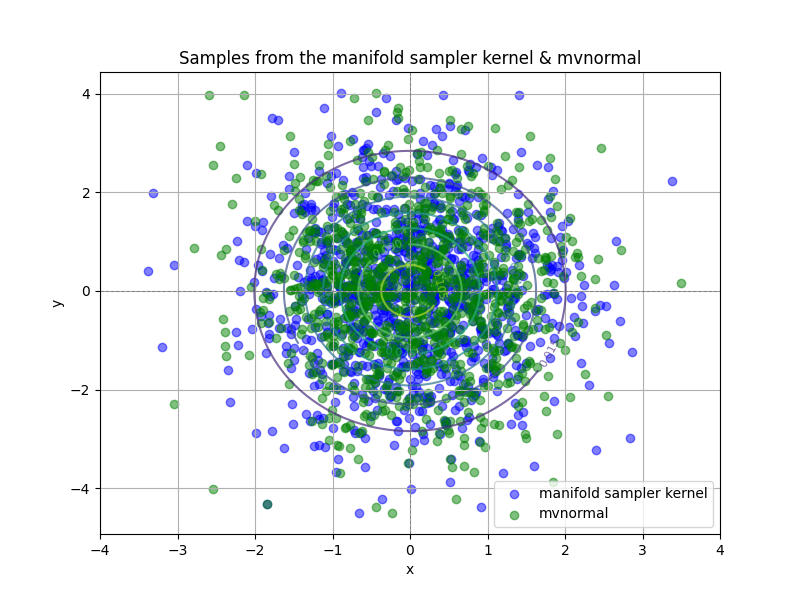
\includegraphics[width=0.6\textwidth, height=0.12\textheight]{scatter.png}
        \caption{distribution scatterplot compare}
        \label{fig:scatter}
    \end{minipage}
    \hspace{0.03\textwidth}
    \begin{minipage}{0.45\linewidth}
        \centering
        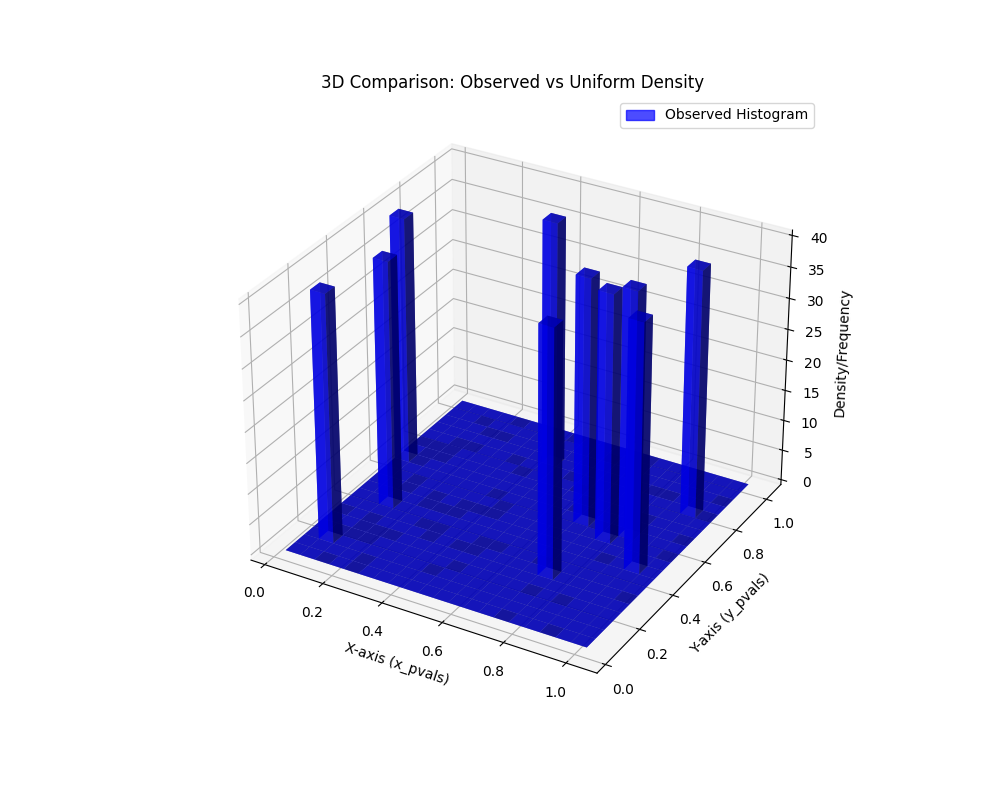
\includegraphics[width=0.6\textwidth, height=0.12\textheight]{pvals.png}
        \caption{distribution of p-value}
        \label{fig:pval}
    \end{minipage}   
\end{figure}





\subsection{Comparison with manifold sampler}
To compare the performance between autostep manifold sampler and usual manifold sampler, we benchmark both samplers from the following perspectives: mixing pattern; auto-correlation (ACF); effective sample size (ESS); time complexity. Regarding the test case, for simplicity we choose $\Mscr$ to be a thin ellipse with constraint equation: $\frac{x^2}{1^2} + \frac{y^2}{0.1^2} = 1$ and set the un-normalized target density to be uniform on $\Mscr$. To see the differences in performance under different initial step sizes, we put $\sigma_0$ in three levels: good, moderate and bad.

\subsubsection{Mixing}
To examine the mixing pattern, we start two chains independently at two ``poles'' of the ellipse: $(1,0)$ and $(-1,0)$ as initial points for each sampler. Moreover, we test both samplers' performances under different initial step size setting: $\sigma = 0.05, 0.1, 0.2$.
% \begin{figure}[H]
%     \centering
%     \begin{adjustbox}{width=\textwidth}
%       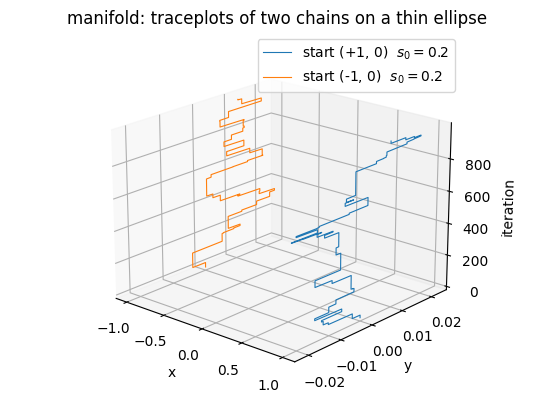
\includegraphics{mixing_bad_s.png}
%       \hspace{0.1em}
%       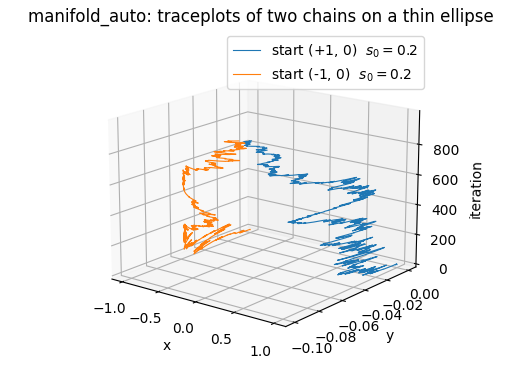
\includegraphics{mixing_auto_bad_s.png}
%       \hspace{0.1em}
%     %   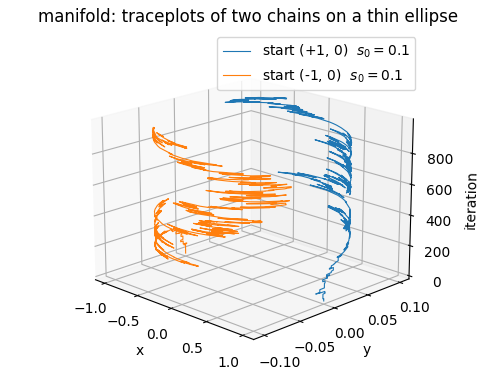
\includegraphics{mixing_margin_s.png}
%     %   \hspace{0.1em}
%     %   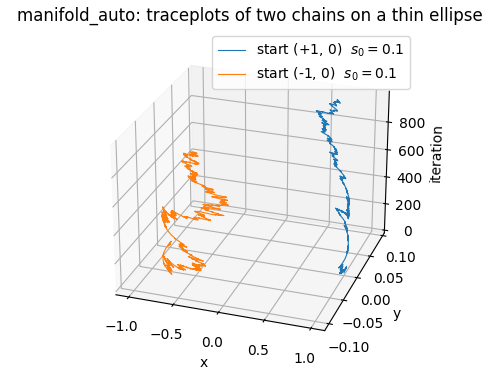
\includegraphics{mixing_auto_margin_s.png}
%     %   \hspace{0.1em}
%       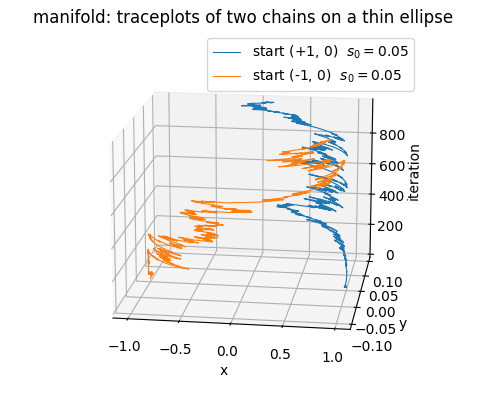
\includegraphics{mixing_good_s.png}
%       \hspace{0.1em}
%       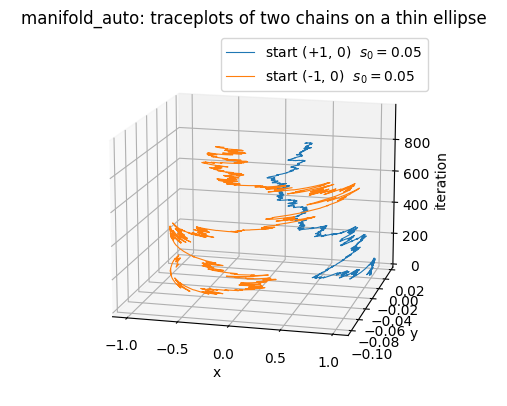
\includegraphics{mixing_auto_good_s.png}
%     \end{adjustbox}
%     \caption{Traceplots of both samplers with different choices of initial step size}
%     \label{fig:mixing}
% \end{figure}

\begin{figure}[H]
    \centering
    \begin{adjustbox}{width=\textwidth}%
      \begin{minipage}[t]{0.48\linewidth}
        \centering
        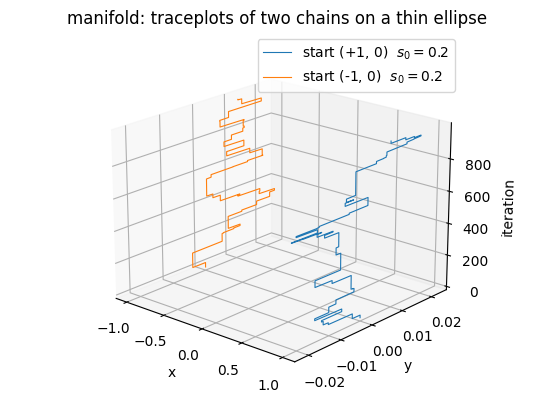
\includegraphics[width=.49\linewidth]{mixing_bad_s.png}\hfill
        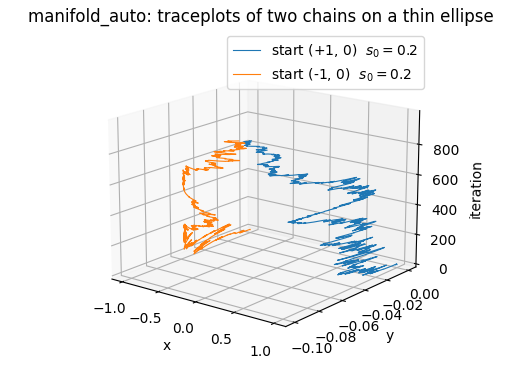
\includegraphics[width=.49\linewidth]{mixing_auto_bad_s.png}
        % \subcaption*{(a) step size = $0.2$}
      \end{minipage}\hfill
      \begin{minipage}[t]{0.48\linewidth}
        \centering
        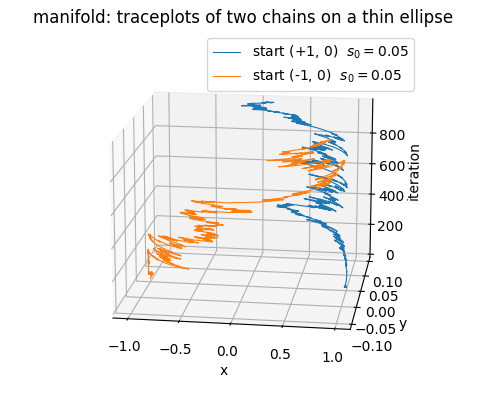
\includegraphics[width=.49\linewidth]{mixing_good_s.png}\hfill
        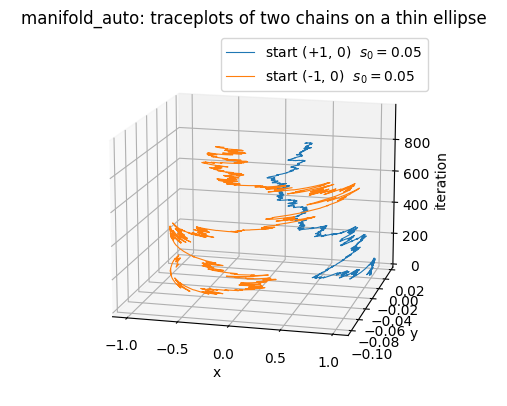
\includegraphics[width=.49\linewidth]{mixing_auto_good_s.png}
        % \subcaption*{(b) step size = $0.05$}
      \end{minipage}
    \end{adjustbox}

    \medskip 
    \begin{adjustbox}{width=0.5\textwidth}%
      \begin{minipage}[t]{\linewidth}
        \centering
        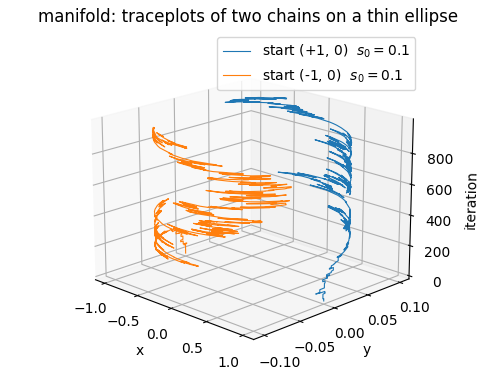
\includegraphics[width=.49\linewidth]{mixing_margin_s.png}\hfill
        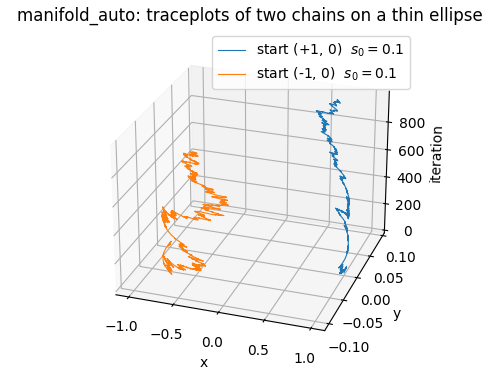
\includegraphics[width=.49\linewidth]{mixing_auto_margin_s.png}
        % \subcaption*{(c) step size = $0.1$}
      \end{minipage}
    \end{adjustbox}
  
    \caption{Traceplots of both samplers with different choices of initial step size}
    \label{fig:mixing}
  \end{figure}
From Figure \ref{fig:mixing}, we can see that both samplers have slow mixing while they still have different mixing patterns under different step size choices. When having a relatively bad choice of initial step size: $\sigma_0 = 0.2$, autostep manifold mixes better than manifold; when under a good/moderate choice of $\sigma_0 = 0.05$ or $0.1$, both performs similarly.


\subsubsection{ACF}
Figure \ref{fig:acf} shows the auto-correlation plot of both samples obtained from both samplers, and it can be observed that under all choices of $\sigma_0$, the acf from autostep manifold samples are lower than that from manifold samples. In particular, when $\sigma_0$ is really bad, the difference between two acfs are even larger.
\begin{figure}[H]
    \centering
    \begin{adjustbox}{width=\textwidth}
      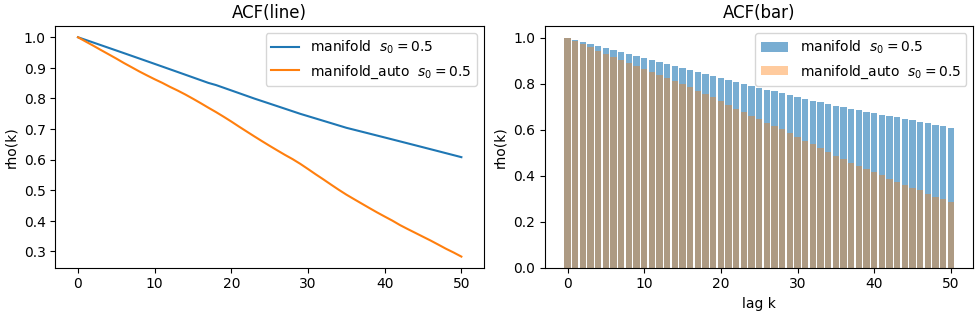
\includegraphics{acf_bad_s.png}
      \hspace{1em}
      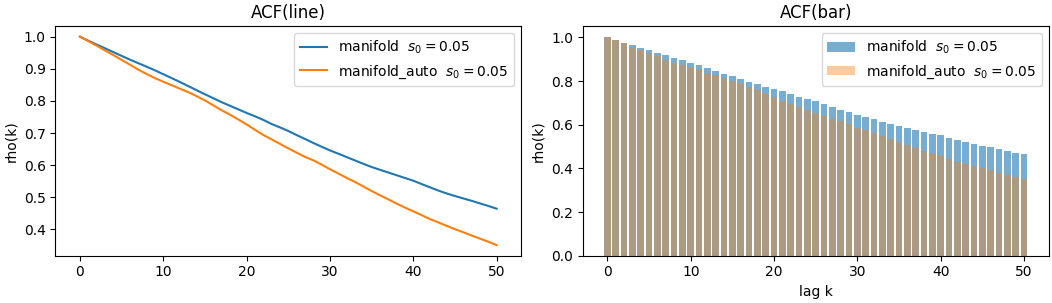
\includegraphics{acf_good_s.png}
      \hspace{1em}
      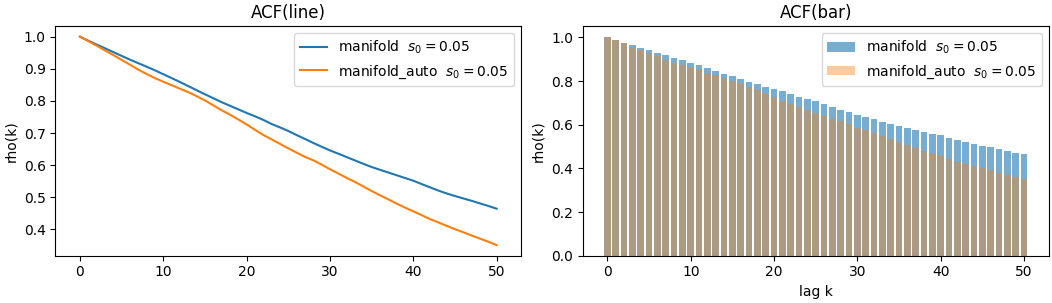
\includegraphics{acf_good_s.png}
    \end{adjustbox}
    \caption{ACF of both samplers with different choices of initial step size}
    \label{fig:acf}
\end{figure}



\subsubsection{ESS}
The ESS formula we are using here is $\frac{N}{1+ 2\sum_{k=1}^K \rho_k}$ where $N$ is the total number of MCMC sample points; $\rho_k$ is the autocorrelation at lag $k$; and $K$ is the maximum lag considered, which in our case, $N = 1000$, $K=50$.
\begin{figure}[H]
    \centering
    \begin{adjustbox}{width=\textwidth}
      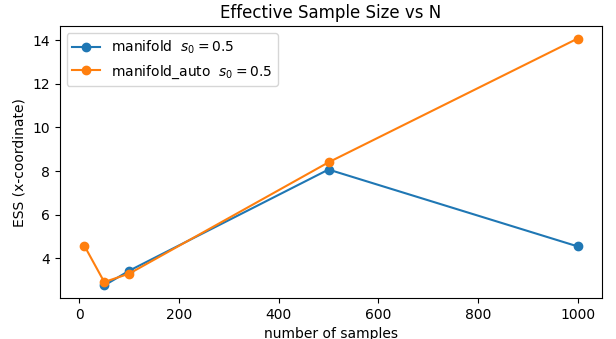
\includegraphics[height=0.06\textheight]{ess_bad_s.png}
      \hspace{1em}
      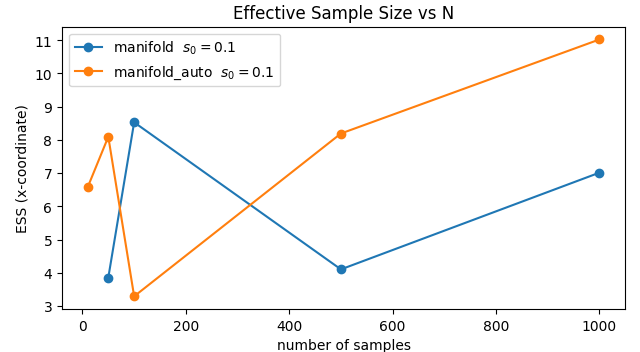
\includegraphics[height=0.06\textheight]{ess_margin.png}
      \hspace{1em}
      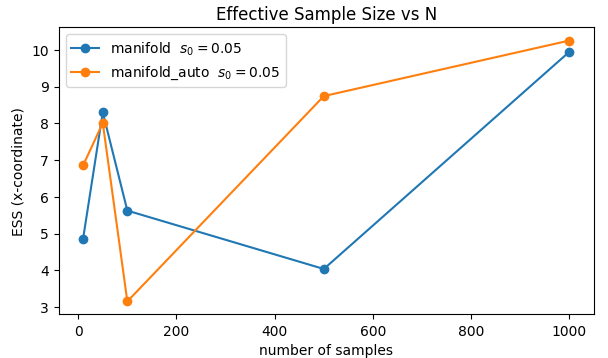
\includegraphics[height=0.06\textheight]{ess_good_s.png}
    \end{adjustbox}
    \caption{ESS of both samplers with different choices of initial step size}
    \label{fig:ess}
\end{figure}
From Figure \ref{fig:ess}, it can be observed that under all choices of $\sigma_0$, the ESS from autostep manifold samples are larger than that from manifold samples when the sample size gets larger. When $\sigma_0$ is bad, ESS from autostep manifold are better at all sample size choices.

\subsubsection{Complexity}
It can be expected that the computational complexity of autostep manifold should be greater than manifold without surprise since the additional step size adjusting step which involves multiple equation solvings within multiple point-projections back to $\Mscr$.
\begin{figure}[H]
    \centering
    \begin{adjustbox}{width=\textwidth}
      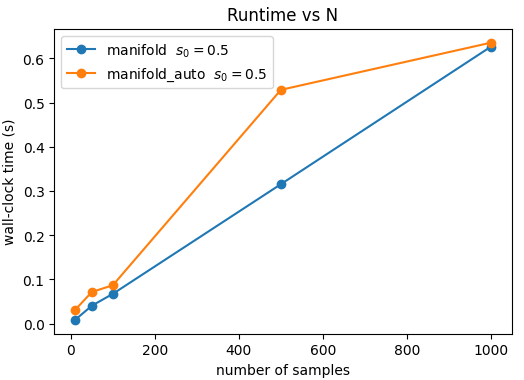
\includegraphics[height=0.05\textheight]{runtime_bad_s.png}
      \hspace{1em}
      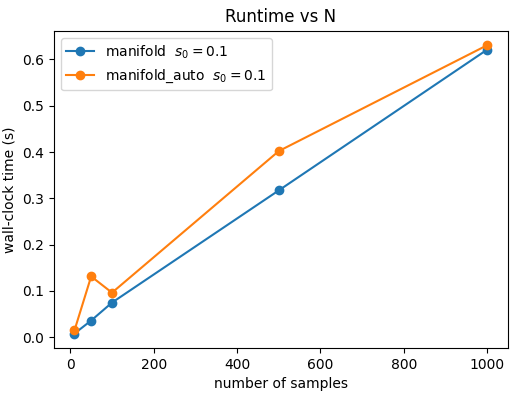
\includegraphics[height=0.05\textheight]{runtime_margin_s.png}
      \hspace{1em}
      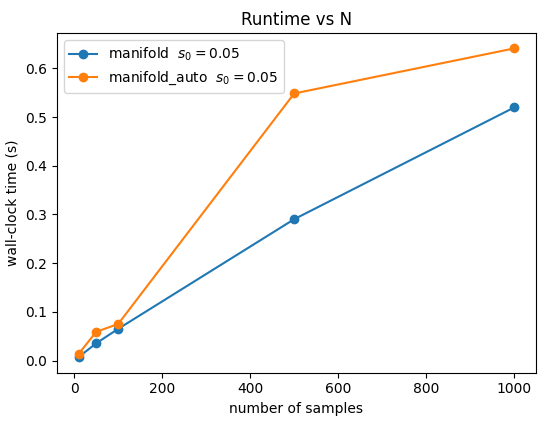
\includegraphics[height=0.05\textheight]{runtime_good_s.png}
    \end{adjustbox}
    \caption{Complexity of both samplers with different choices of initial step size}
    \label{fig:time}
\end{figure}
So Figure \ref{fig:time} justifies our expectation that under all step size choices, the time complexity of autostep manifold is greater than manifold at all levels of sample size.



\section{Conclusion}
In this project, we modified the traditional manifold sampler(RATTLE scheme) with the autostep adjustment and discussed its correctness and benchmarked its performance against the traditional one. We should point out that though autostep manifold sampler is valid and it performs slightly better than the traditional manifold sampler in some cases, it however does not show much advantage compared to the other, especially when the initial step size is well-chosen, and both samplers do not appear to have fast mixing in our test case.

For future directions, there are certainly some aspects that remain to be explored further. First, some cases with non-trivial distributions defined on $\Mscr$ should be considered to evaluate whether autostep manifold outperforms much more than the traditional one; Second, the complexity of autostep manifold is still a big issue. In high-dimensional cases, it could probably take ages to run the samplerby simple computing capacity. So whether it is a scalable method needs to be explored further; Lastly and more challengingly, devise another novel sampler that is even more robust to the choice of step size parameter. Initial conjecture sketches that one could be contour and gradient-based.





\nocite{*}



\newpage

\bibliography{ref}


\clearpage
\appendix
\begin{center}
{\LARGE \textbf{Appendix}}  
\end{center}
\renewcommand{\thefigure}{\thesection.\arabic{figure}}
\renewcommand{\thetable}{\thesection.\arabic{table}}
\setcounter{figure}{0}  % Reset figure counter
\setcounter{table}{0}   % Reset table counter
\setcounter{algorithm}{0}  % Reset algorithm counter



\section{Proofs}
\begin{proof}[Proof of Lemma \ref{lemma:finte_solver}]
Since $\Mscr$ is smooth, then $F$ is continuous. Hence $\exists \delta > 0$ such that $\norm{x' - x} < \delta$, we have $\norm{F(x') - F(x)} < \eps$. Therefore for fixed $\sigma_0$ and $v_x$, $\exists n \in \N$ and $c \in \R^m$ such that $\norm{\sigma_0 2^{-n} v_x + Q_x \cdot c} < \delta$. Put $x' = x + \sigma_0 2^{-n} v_x + Q_x \cdot c$. Note that $F(x) = 0$, hence $\norm{F(x + \sigma_0 2^{-n} v_x + Q_x \cdot c)} < \eps$ implying $N \leq n < \infty$.


% Let $G(c) = F(x + v_x + Q_x\cdot c)$, then by quasi-Newton, \[c_{n+1} = c_n - (\nabla G)^{-1}G(c_n)\]where $\nabla G = Q_x^\top Q_x$ is constant w.r.t $c$. Suppose $c^*$ is the solution to $G(c) = 0$, then
% \[0 = G(c^*) = G(c_n) + \nabla G (c^* - c_n) + o(c^* - c_n)\]
% This implies: $c^* - c_{n+1} = - (\nabla G)^{-1} o(c^* - c_n)$. Hence $c_n \to c^*$. Since $\Mscr$ is smooth, so $G$ is continuous, hence $\exists N \in \N$ and $\delta > 0$ such that $\norm{c_N - c^*} < \delta$, we have $\norm{G(c_N) - G(c^*)} < \eps$.

\end{proof}


\begin{proof}[Proof of Proposition \ref{prop:invariance}]
Since manifold sampler with augmented state: $(x, v_x)$ is $\pi$-invariant by \cite{manifoldparent}, then apply the arguments in the proof of Proposition $4.2$ in \cite{autostep}
\end{proof}


% \begin{proof}[Proof of Theorem \ref{thm:ratest}]
% At each iteration, we first simulate a random ``altitude'' $Y_i|=g(X), X$ and generate a sequence of samples from autostep manifold on the contour given the ``altitude'' and pick the last one. 
% We introduce another random variable $Y$, which represents the random ``altitude'' of $g$ evaluated at some point $x \in \R^n$. 

% Suppose we have a contour of $g$: $\Gamma_y = \inv{g}(\{y\})$ and we run manifold sampler on that to obtain a chain: $\{X_1, \ldots, X_m\}$. Cosnider the probability measure of $X_1$ w.r.t Lebesgue measure:
% \[\P(X_1 \in A)= \mu(A) = \int_A g(x)dx = \int_{\R^+} \P(X_1\in A | Y = y) f_Y(y) dy\]
% While by co-area formula, \[\int_A g(x) dx = \int_{\R} \int_{A \cap g^{-1}(\{y\})} \frac{g(x)}{\abs{\nabla g(x)}} \Hcal^{n-1}(dx)dy\]

% % So the probability measure of $X_1$ is:
% % \[\P(X_1 \in A)= \mu(A) = \int_A g(x)dx = \int_{\R^+} \P(X_1\in A | Y = y) dy\] 
% So we can put the conditional probability measure: \[\xi_Y(A) = \P(X_1 \in A | Y = y) = \int_{A \cap g^{-1}(\{y\})} \frac{g(x)}{\abs{\nabla g(x)} f_Y(y)} \Hcal^{n-1}(dx)\]where the density for the ``altitude'' $Y$ is: \[f_Y(y) = \int_{g^{-1}(\{y\})} \frac{g(x)}{\abs{\nabla g(x)}} \Hcal^{n-1}(dx)\]

% The key properties from the above derivations are:
% \begin{enumerate}
% \item[i]
% $X_1 \sim \mu$ is equivalent to $Y \sim \nu$ and $X_1 | Y \sim \xi_Y$
% \item[ii]
% If the manifold sampler kernel $K$ we want to test leads to invariant distribution with respect to $\xi_Y$, i.e. $\xi_Y(A) = \int \xi_Y(dx) K(x, A)$, then given $X_2 |X_1 \sim K(X_1, \cdot)$, we will have $X_2 \sim \mu$. This is because $X_2 | Y \sim \xi_Y$ and $Y \sim \nu$, which is equivalent to $X_2 \sim \mu$. Finally, by induction we can have $X_m \sim \mu$. Put $S = X_m$ as our test sample.
% \end{enumerate}
% In short, if we test: $S \sim \mu$, then $K$ is correct; if not, then $K$ has bug. So to test if $S \sim \mu$, once we have a sequence of test samples generated by our test algorithm, and another sequence of samples directly generated from the true distribution: $\mu$ with density $g$, then we could use Kolmogorov-Smirnov test to check the p-value. If p-value is small, then we reject $H_0: S \sim \mu$.
% \end{proof}

\section{Additional pseudo-codes}
Below are some more pseudo-codes that have been used in the project, some of which are based on efficient tricks of matrix computation

\begin{algorithm}[H]
    \caption{Quasi-Newton solver}
    \label{algo:solver}
    \begin{algorithmic}
    \Require $x+v_x$, $Q_x$ and $L_x$
    \State $a \gets \mathbf{0}$
    \State $y \gets x+v_x + Q_x \cdot a$; 
    \State $i \gets 1$
    \State found $\gets$ False
    
    \While{$i <$ nmax and $\norm{F(y)} > \eps$}
         \State Forward-backward solve: $L_x L_x^\top \delta_a = -\norm{F(y)}$ for $\delta_a$
         \State $a \gets a + \delta_a$ 
         \State $y \gets x+v_x + Q_x \cdot a$
         \State $i \gets i+1$
    \EndWhile
    \If {$i < $nmax}
    \State found $\gets$ True
    \EndIf
    \State\Return $(y, \text{found})$
    
    % \For{$i = 1, \ldots, n$}
    %     \State sample: $x' \sim q(\cdot | x)$
    % \EndFor
    \end{algorithmic}
\end{algorithm}


\begin{algorithm}[H]
    \caption{Forward tangent move: sample $v_x \in T_x$}
    \label{algo:forward tangent}
    \begin{algorithmic}
    \State Generate $n$-dimensional i.i.d $z = \{z_i\}_{i=1}^n$ where $z_i \sim N(0,1), \forall i$ 
    \State Forward-backward solve for $\xi$: $L_x L_x^\top \xi= Q_x^\top z$
    \State Tangent proposal by projecting to tangent space: $v_x \gets \mathbf{P}_{T_x} \cdot z = (\mathbb{I} - Q_x(Q_x^\top Q_x)^{-1} Q_x^\top) \cdot z = z - Q_x \xi$ 
    \end{algorithmic}
\end{algorithm}

\begin{algorithm}[H]
    \caption{Reverse tangent move: $v_y \in T_y$}
    \label{algo:reverse tangent}
    \begin{algorithmic}
    \State Find Cholesky decomposition of $L_y L_y^\top = Q_y^\top Q_y$
    \State Forward-backward solve for $\xi$: $L_y L_y^\top \xi= Q_y^\top (x-y)$
    \State Set reverse tangent proposal: $v_y \gets \mathbf{P}_{T_y} \cdot (x-y) = (\mathbb{I} - Q_y(Q_y^\top Q_y)^{-1} Q_y^\top) \cdot (x-y) = (x-y) - G_y \xi$
    \end{algorithmic}
\end{algorithm}

\section{Additional experiment results}

\begin{table}[H]
    \centering
    \begin{tabular}{|c|c|}
    \hline
    \textbf{$x$ component} & \textbf{$y$ component} \\
    \hline
    0.7946637387576738 & 0.5005673707894058 \\
    0.9136894237272155 & 0.7946637387576738 \\
    0.06153429181321559 & 0.14836452078962484 \\
    0.8282194040312439 & 0.5728904395829821 \\
    0.7228251828701066 & 0.28779764348473313 \\
    0.9357699014782725 & 0.4006338815832625 \\
    0.025633868930359294 & 0.6101664688189142 \\
    0.43260886958153144 & 0.8282194040312439 \\
    0.1082872208757189 & 0.37012017606173 \\
    0.6854967337920594 & 0.5728904395829821 \\
    \hline
    \end{tabular}
    \caption{P-values of $x$ and $y$ components in K-S test for correctness}
    \label{tab:pvals}
    \end{table}
Table \ref{tab:pvals} shows the p-values of both $x$ and $y$ components during the K-S test mentioned in section $4.1$. As we can see that all values are above the adjusted threshold $0.025$ by realtively big margin, indicating the $H_0$ should not be rejected.
% \begin{table}[H]
%     \centering
%     \begin{minipage}{0.48\textwidth}
%         \centering
%         \resizebox{\textwidth}{!}{
%         \begin{tabular}{|rlrrr|}
%             \hline
%            & Type & Estimate & Std. Error & t value \\ 
%             \hline
%           (Intercept) & Fixed & -0.12 & 0.06 & -2.00\\ 
%             FormDistractor & Fixed & 0.37 & 0.04 & 10.51\\ 
%             MeaningDistractor & Fixed & 0.12 & 0.04 & 3.47\\ 
%             Mandarin\_AoA & Fixed & 0.28 & 0.08 & 3.73\\ 
%             cs\_score & Fixed & -0.14 & 0.06 & -2.24\\ 
%             lextale\_man & Fixed & -0.24 & 0.09 & -2.83\\ 
%             dominance & Fixed & -0.01 & 0.09 & -0.11\\ 
%             (Intercept) & Random & 0.36 & - & - \\ 
%             (Residual) & Random & 0.79 & - & - \\ 
%              \hline
%           \end{tabular}
%         }
%           \caption{Summary of fixed and random effects of RT model}
%           \label{tab:RT model summary}
%     \end{minipage}
%     \hfill
%     \begin{minipage}{0.48\textwidth}
%         \centering
%         \resizebox{\textwidth}{!}{
%         \begin{tabular}{|rlrrr|}
%             \hline
%            & Type & Estimate & Std. Error & z value\\ 
%             \hline
%           (Intercept) & Fixed & 2.79 & 0.14 & 20.28\\ 
%             dominance & Fixed & -0.77 & 0.16 & -4.91\\ 
%             FormDistractor & Fixed & -1.55 & 0.14 & -11.14 \\ 
%             MeaningDistractor & Fixed & -1.13 & 0.14 & -7.96 \\ 
%             Mandarin\_AoA & Fixed & -0.40 & 0.13 & -3.17 \\ 
%             cs\_score & Fixed & 0.28 & 0.11 & 2.57 \\ 
%             lextale\_eng & Fixed & 0.31 & 0.13 & 2.37 \\ 
%             (Intercept) & Random & 0.53 & - & - \\ 
%              \hline
%           \end{tabular}
%         }
%           \caption{Summary of fixed and random effects of accuracy model}
%           \label{tab:accuracy model summary}
%     \end{minipage}
% \end{table} 


% Now with combining autostep But we notice that such algorithms along with many others with deterministic proposals have things in common, which is that they usually have involutive transformation between states to satisfy the reversibility. In MCMC literature, \cite{tierney1998} pointed out that if the transformation between states is deterministic and involutive, then by setting the proposal to be delta measure, the detailed balance condition will follow, which implies the distribution invariance. So we wish to take advantage of this involution framework to show that the manifold sampler has $\pi$ invariance.

% Before that, we will show some important results as a baseline for our justification for $\pi$ invariance of the manifold sampler. Suppose the target distribution is $\pi$ with density $f$ with respect to the Lebesgue measure, and let $x, y$ be the current and next state. The usual Metropolis-Hastings ratio is: $r = \frac{f(y) q(x | y)}{f(x) q(y | x)}$ for some proposal: $q$. But given our state transformation $T$ such that $y = T(x)$ being deterministic and involutive, i.e. $T = \inv{T}$, then $r(x) = \frac{f(T(x))}{f(x)} \cdot \abs{J_T(x)}$, where $J_T(x)$ is the determinant of Jacobian matrix of $T$. Now we extend this notation a little bit:

% Suppose our target distribution $\pi$ is defined w.r.t. measure $\mu$ so that the Radon-Nikodyn derivative: $\frac{d\pi}{d\mu}$ is well-defined, then we define the ratio: \[r(x) = \frac{d T^*\pi}{d\mu}(x) / \frac{d\pi}{d\mu}(x)\]where $T^*\pi$ is the pull-back probability measure such that: $T^*\pi(A) = \pi(T(A))$

% If we apply the M-H routine with the new $r(x)$ defined above, then the consequence is that we will have global balance and hence distribution invariance. To show this result, we will introduce the following lemma as an intermediate step.

% % \begin{lemma}\label{lemma_invol}
% % Let $\pi$ be the target distribution on $\Xcal$ with respect to measure $\mu$ and $T$ be an involution on $\Xcal$. Given the current state: $x$ and the next state: $y$ such that $y = T(x)$, and the acceptance probability is defined as:  
% % \[\alpha(x, T(x)) = \min\{1, r(x)\}\]
% % then we will have the detailed balance equation: 
% % \[\frac{d\pi}{d\mu}(x) \cdot \alpha(x, T(x)) = \frac{d T^*\pi}{d\mu}(x)\cdot\alpha(T(x), x)\]
% % \end{lemma}

% % \begin{proof}
% % First, note that by the definition of pull-back measure, $\frac{d\pi}{d\mu}(y) = \frac{d\pi}{d\mu}(T(x)) = \frac{d T^*\pi}{d\mu}(x)$. Since $T = T^{-1}$, then $x = T^{-1}(y) = T(y)$, so again, $\frac{d\pi}{d\mu}(x) = \frac{d\pi}{d\mu}(T(y)) = \frac{d T^*\pi}{d\mu}(y)$, hence $r(x) \cdot r(y) = 1$.

% % Therefore, \begin{align*}
% % & \frac{d\pi}{d\mu}(x) \cdot \alpha(x, T(x)) = \frac{d T^*\pi}{d\mu}(x) \cdot \min\Big\{\frac{d\pi}{d\mu}(x) / \frac{d T^*\pi}{d\mu}(x), 1\Big\}\\
% % & = \frac{d T^*\pi}{d\mu}(x) \cdot\min\Big\{\frac{1}{r(x)}, 1\Big\} = \frac{d T^*\pi}{d\mu}(x) \cdot\min\{r(y), 1\} = \frac{d T^*\pi}{d\mu}(x)\cdot\alpha(T(x), x)
% % \end{align*}

% % \end{proof}


% % \begin{theorem}\label{thm_invariance}
% % Let $X$ be the current state and $Y$ be the next state and $X$ has distribution: $\pi$ which has density with respect to measure $\mu$. Suppose $T$ is an involution such that $Y = T(X)$. Define the transition kernel: $K(x, E) = \alpha \cdot \1_E(T(x)) + (1 - \alpha) \1_E(x)$ for any event $E$. Then the global balance holds:
% % \[\P(Y \in A) = \pi(A) = \int_{x \in \Xcal} \pi(dx) K(x, A)\]
% % \end{theorem}

% % \begin{proof}
% % \begin{align*}
% % & \int_{x \in \Xcal} \pi(dx) K(x, A) = \int_{x \in \Xcal} \pi(dx) [\alpha\1_A(T(x)) + (1-\alpha)\1_A(x)]\\
% % & = \int_{x \in \Xcal} \pi(dx) \alpha(x, T(x)) \1_A(T(x)) + \int_{x \in \Xcal} \pi(dx) (1 - \alpha) \1_A(x)\\
% % & = \int_{x \in \Xcal} \frac{d T^*\pi}{d\mu}(x) \alpha(T(x), x)\1_A(T(x)) d\mu(x) + \int_{x \in \Xcal} \pi(dx) (1 - \alpha) \1_A(x)\\
% % & = \int_{y \in \Xcal} \pi(dy) \alpha(y, \inv{T}(y)) \1_A(y) + \int_{x \in \Xcal} \pi(dx) (1 - \alpha) \1_A(x)\\
% % & = \int_{y \in \Xcal} \pi(dy) \alpha(y, T(y)) \1_A(y) + \int_{x \in \Xcal} \pi(dx) (1 - \alpha) \1_A(x)\\
% % & = \int_{y \in \Xcal} \pi(dy) \1_A(y) = \pi(A)\\
% % \end{align*}
% % \end{proof}





% \subsection{Involution within the manifold sampler}
% Now back to the manifold sampler setting, compared to \cite{manifoldparent}, the advantage of the above abstract framework is that it is a good tool to help us prove that the manifold sampler has $\pi$ invariance if we can find an involution between the states. Indeed, by the trick of augmenting space, i.e. introducing some necessary auxiliary variables, we can construct an involution from the manifold sampler.

% Let $S = \{(x, v_x) \in T\mathscr{M} : \norm{F(x + v_x + G_x \cdot a)} < \eps\} \subset T\mathscr{M}$ for some small enough positive $\eps$, where $w_x = G_x \cdot a \in N_x$, for some coefficient vector $a \in \R^m$. This means $S$ is some subset of tangent bundle $T\mathscr{M}$ such that we could have a successful projection on $\mathscr{M}$, thus we could denote $y = x + v_x + w_x$. 
% % For simplicity, we will consider all the states from $S$ for later discussion.

% Define $T_0: T\mathscr{M} \to T\mathscr{M}$ as $T_0(x, v_x) = (y, v_y)$ 
% where:
% $\begin{cases}
% y =  x + v_x + w_x = x + v_x + G_x \cdot a\\
% v_y = \textit{proj}_{T_y}(x-y)
% \end{cases}$

% Let $A = \{(x, v_x) \in S : \norm{F(y + v_y + G_y a'} < \eps\}$, where $(y, v_y) = T_0(x, v_x)$, so $A$ represents the set where reversibility holds.

% Define $T: T\mathscr{M} \to T\mathscr{M}$ as $T(x, v_x) = T_0(x, v_x) \cdot \1_A + I(x, v_x) \cdot \1_{A^c}$.

% We claim that: $T$ is a non-trivial involution on $T\mathscr{M}$, i.e. $T \neq I$.

% \begin{proof}
% First, it is essential to argue that such $A \neq \emptyset$. By assumption, $\mathscr{M}$ is smooth manifold so that $F$ is a smooth function. Thus, for a given $\eps > 0, \exists \delta > 0$ such that $\forall x',x \in \R^n$ with $\norm{x'- x} < \delta$, we have $\norm{F(x') - F(x)} < \eps$. 

% In order to find at least one element, we could pick $x \in \mathscr{M}$, and choose an open ball inside the ambient space centered at $x$ : $B_\delta(x)$ with radius $\delta$, and pick $y \in B_\delta(x) \cap \mathscr{M}$.

% Let $v_x = \textit{proj}_{T_x}(y-x)$, so during the process of solving $a$ with starting $a_0 = 0$, for each intermediate $a$, 
% \[\norm{x + v_x + G_x a - x} \leq \norm{v_x + \textit{proj}_{N_x}(y-x)} = \norm{y-x} < \delta\]hence $x + v_x + G_x a \in B_\delta(x)$, which implies $\norm{F(x + v_x + G_x a)} < \eps$, so $(x, v_x) \in S$;

% Now for the reverse projection, by the similar argument from above, for each intermediate $a'$, \[\norm{y + v_y + G_y a' - y} \leq \norm{v_y + \textit{proj}_{N_y}(x-y)} = \norm{x-y} < \delta\]hence $y + v_y + G_y a' \in B_\delta(y)$, which implies $\norm{F(y + v_y + G_y a')} < \eps$, so $(x, v_x) \in A$.
% % so \[v_x = (I - G_x(G_x^TG_x)^{-1}G_x^T)(y-x)\]thus \[F(x + v_x + G_x \cdot a) = F(y + G_x(a - (G_x^TG_x)^{-1}G_x^T(y-x)))\]
% % Let coefficient $b = (G_x^TG_x)^{-1}G_x^T(y-x)$, choose $a$ such that $\norm{a - b} < \frac{\delta}{\norm{G_x}}$, then
% % \[\norm{y + G_x(a-b) - y} \leq \norm{G_x} \cdot \norm{a-b} < \delta\]
% % hence $y + G_x(a-b) \in B_\delta(y)$, which implies that $\norm{F(x + v_x + G_x \cdot a)} < \eps$ since $F(y) = 0$, so $(x, v_x) \in S$.

% % By the similar arugment for the reverse projection, we let $b' = (G_y^TG_y)^{-1}G_y^T(x-y)$, thus $y + v_y + G_y a' = x + G_y(a'-b')$. So we could choose $a'$ with $\norm{a'- b'} < \frac{\delta}{\norm{G_y}}$, thus $y + v_y + G_y a' \in B_\delta(x)$ and hence $\norm{F(y + v_y + G_y a')}< \eps$. So $(x, v_x) \in A$.

% Next we will show that by the definition of $T_0$, $\forall (x, v_x) \in A, T_0 \circ T_0 = I$. 

% Let $(x, v_x) \in A$. Suppose $(y, v_y) = T_0(x, v_x)$ and $(x', v_{x'}) = T_0(y, v_y) = T_0\circ T_0(x, v_x)$.

% Then by definition, 
% \[x' = y + v_y + w_y = y + \textit{proj}_{T_y}(x-y) + \textit{proj}_{N_y}(x-y) = y + (x - y) = x\]and
% \[v_{x'} = \textit{proj}_{T_{x'}}(y-x') = \textit{proj}_{T_x}(y-x) = \textit{proj}_{T_x}(v_x + w_x) = v_x \text{ (since $w_x \perp T_x$)}\]
% which proves our claim.
% \end{proof}





% \begin{corollary}
% Let $\pi$ be the distribution defined on the manifold. Let the kernel of the manifold sampler be:
% \[K(\tilde{x}, A) = \alpha\Big(\tilde{x}, T(\tilde{x})\Big)\1_A(T(\tilde{x})) + \Big(1- \alpha(\tilde{x}, T(\tilde{x}))\Big)\1_A(\tilde{x})\]where $\tilde{x} = (x, v_x)$ and $\tilde{y} = (y, v_y)$ for the augmented space, and \[\alpha\Big(\tilde{x}, T(\tilde{x})\Big) = \min\Big\{1, \frac{f(y)p(v_y|y)}{f(x)p(v_x|x)}\Big\}\]
% then $K$ has distribution invariance.
% \end{corollary}


\end{document}

